\documentclass{beamer}
\usepackage[utf8]{inputenc}

\usetheme{Madrid}
\usecolortheme{default}
\usepackage{extarrows}
\usepackage{amsmath}
\usepackage{extarrows}
\usepackage{amssymb,amsfonts,amsthm}
\usepackage{txfonts}
\usepackage{tkz-euclide}
\usepackage{listings}
\usepackage{adjustbox}
\usepackage{array}
\usepackage{tabularx}
\usepackage{gvv}
\usepackage{lmodern}
\usepackage{circuitikz}
\usepackage{tikz}
\usepackage{graphicx}
\usepackage{amsmath} 

\setbeamertemplate{page number in head/foot}[totalframenumber]

\usepackage{tcolorbox}
\tcbuselibrary{minted,breakable,xparse,skins}

\definecolor{bg}{gray}{0.95}
\DeclareTCBListing{mintedbox}{O{}m!O{}}{%
  breakable=true,
  listing engine=minted,
  listing only,
  minted language=#2,
  minted style=default,
  minted options={%
    linenos,
    gobble=0,
    breaklines=true,
    breakafter=,,
    fontsize=\small,
    numbersep=8pt,
    #1},
  boxsep=0pt,
  left skip=0pt,
  right skip=0pt,
  left=25pt,
  right=0pt,
  top=3pt,
  bottom=3pt,
  arc=5pt,
  leftrule=0pt,
  rightrule=0pt,
  bottomrule=2pt,
  toprule=2pt,
  colback=bg,
  colframe=orange!70,
  enhanced,
  overlay={%
    \begin{tcbclipinterior}
    \fill[orange!20!white] (frame.south west) rectangle ([xshift=20pt]frame.north west);
    \end{tcbclipinterior}},
  #3,
}
\lstset{
    language=C,
    basicstyle=\ttfamily\small,
    keywordstyle=\color{blue},
    stringstyle=\color{orange},
    commentstyle=\color{green!60!black},
    numbers=left,
    numberstyle=\tiny\color{gray},
    breaklines=true,
    showstringspaces=false,
}
\title %optional
{5.13.58}


\author 
{Kartik Lahoti - EE25BTECH11032}



\begin{document}


\frame{\titlepage}
\begin{frame}{Question}
Let $\omega \neq 1$ be a cube root of unity and $\mathbb{S}$ be the set of all non-singular matrices of the form 

\begin{align}
    \myvec{1 & a & b \\ \omega & 1 & c \\ \omega^2 & \omega & 1}
\end{align}

where each of $a,b$ and $c$ is either $\omega$ or $\omega^2$. Then the number of distinct matrices in the set $\mathbb{S}$ is
\end{frame}

\begin{frame}{Theoretical Solution}
Let,

\begin{align}
    \vec{A} = \myvec{1 & a & b \\ \omega & 1 & c \\ \omega^2 & \omega & 1}
\end{align}

where $\vec{A} \in \mathbb{S}$

For $\vec{A}$ to be Non-singular , $\vec{A}$ should be a full rank matrix.
\end{frame}

\begin{frame}{Theoretical Solution}
Thus, 
\begin{align}
    rank\brak{\vec{A}} = 3 
\end{align}


\begin{align}
    \myvec{1 & a & b \\ \omega & 1 & c \\ \omega^2 & \omega & 1} \xleftrightarrow[]{R_2\rightarrow R_2 - \omega R_1 }\myvec{1 & a & b \\ 0 & 1-a\omega & c-b\omega \\ \omega^2 & \omega & 1}
\end{align}
\end{frame}

\begin{frame}{Theoretical Solution}
\begin{align}
    \myvec{1 & a & b \\ 0 & 1-a\omega & c-b\omega \\ \omega^2 & \omega & 1} \xleftrightarrow[]{R_2\rightarrow R_2 - \omega^2 R_1 }\myvec{1 & a & b \\ 0 & 1-a\omega & c-b\omega \\ 0 & \omega - a\omega^2 & 1-b\omega^2}
\end{align}

\begin{align}
    \myvec{1 & a & b \\ 0 & 1-a\omega & c-b\omega \\ 0 & \omega - a\omega^2 & 1-b\omega^2} \xleftrightarrow[]{R_3\rightarrow R_3 - \omega R_2 }\myvec{1 & a & b \\ 0 & 1-a\omega & c-b\omega \\ 0 & 0 & 1-c\omega}
\end{align}
\end{frame}

\begin{frame}{Theoretical Solution}

For this Row Reduced Echelon Form Matrix to be a full rank matrix, 
the diagonal pivots should be non-zero.

\begin{align}
    1-c\omega \neq 0 \implies c = \omega
\end{align}
\begin{align}
    1-a\omega \neq 0 \implies a = \omega
\end{align}
\end{frame}
\begin{frame}{Theoretical Solution}
Non-singularity does not depends on $b$ thus, $b \in \cbrak{\omega , \omega^2} $

\begin{align}
    \therefore n\brak{\mathbb{S}} &= 1 \times 2 \times 1 \\
               n\brak{\mathbb{S}} &= 2
\end{align}

Hence , number of Matrices in Set $\mathbb{S}$ is $2$.

\end{frame}

\begin{frame}[fragile]
    \frametitle{C Code - Line Generator  }
    \begin{lstlisting}
void linegen(double *X, double *Y , double *Z , double *A , double *B , int n , int m )
{
    double temp[m] ; 
    for (int i = 0 ; i < m ; i++)
    {
        temp [ i ] = (B[i]- A[i]) /(double) n ; 
    }
    for (int i = 0 ; i <= n ; i++ )
    {
        X[i] = A[0] + temp[0] * i ; 
        Y[i] = A[1] + temp[1] * i ;
        Z[i] = A[2] + temp[2] * i ; 
    }
}
\end{lstlisting}
\end{frame}

\begin{frame}[fragile]
    \frametitle{Python Code - 1 }
    \begin{lstlisting}
import ctypes
import numpy as np
import matplotlib.pyplot as plt

i = 1 
def line_cre(P: np.ndarray , Q: np.ndarray, str):
    handc1 = ctypes.CDLL("./line_gen.so")
    global i 
    handc1.linegen.argtypes = [
        ctypes.POINTER(ctypes.c_double),
        ctypes.POINTER(ctypes.c_double),
        ctypes.POINTER(ctypes.c_double),
        ctypes.POINTER(ctypes.c_double),
        ctypes.POINTER(ctypes.c_double),
        ctypes.c_int , ctypes.c_int
    ]
    handc1.linegen.restype = None

\end{lstlisting}
\end{frame}

\begin{frame}[fragile]
    \frametitle{Python Code}
    \begin{lstlisting}
n = 200
    X_l = np.zeros(n,dtype=np.float64)
    Y_l = np.zeros(n,dtype=np.float64)
    Z_l = np.zeros(n,dtype=np.float64)
    handc1.linegen (
        X_l.ctypes.data_as(ctypes.POINTER(ctypes.c_double)),
        Y_l.ctypes.data_as(ctypes.POINTER(ctypes.c_double)),
        Z_l.ctypes.data_as(ctypes.POINTER(ctypes.c_double)),
        P.ctypes.data_as(ctypes.POINTER(ctypes.c_double)),
        Q.ctypes.data_as(ctypes.POINTER(ctypes.c_double)),
        n,3
    )
\end{lstlisting}
\end{frame}
\begin{frame}[fragile]
    \frametitle{Python Code}
    \begin{lstlisting}
    if i == 1 :
        ax.plot([X_l[0],X_l[-1]],[Y_l[0],Y_l[-1]],[Z_l[0],Z_l[-1]],str,label = "Correct Solution" )
    elif i == 2 : 
        ax.plot([X_l[0],X_l[-1]],[Y_l[0],Y_l[-1]],[Z_l[0],Z_l[-1]],str,label = "Incorrect Solution" )
    else :
        ax.plot([X_l[0],X_l[-1]],[Y_l[0],Y_l[-1]],[Z_l[0],Z_l[-1]],str)
    i=i+1
\end{lstlisting}
\end{frame}

\begin{frame}[fragile]
    \frametitle{Python Code}
    \begin{lstlisting}
fig = plt.figure()

ax = fig.add_subplot(111,projection="3d")
# let omega correspond to 1 and omega square to -1 
O = np.zeros(3,dtype=np.float64).reshape(-1,1)
p1 = np.array([1,1,1],dtype=np.float64).reshape(-1,1)
p2 = np.array([-1,1,1],dtype=np.float64).reshape(-1,1)
p3 = np.array([1,-1,1],dtype=np.float64).reshape(-1,1)
p4 = np.array([1,1,-1],dtype=np.float64).reshape(-1,1)
p5 = np.array([1,-1,-1],dtype=np.float64).reshape(-1,1)
p6 = np.array([-1,1,-1],dtype=np.float64).reshape(-1,1)
p7 = np.array([-1,-1,1],dtype=np.float64).reshape(-1,1)
p8 = np.array([-1,-1,-1],dtype=np.float64).reshape(-1,1)
\end{lstlisting}
\end{frame}
\begin{frame}[fragile]
    \frametitle{Python Code}
    \begin{lstlisting}
line_cre(p1,O,"g-")
line_cre(p2,O,"r-")
line_cre(p3,O,"g-")
line_cre(p4,O,"r-")
line_cre(p5,O,"r-")
line_cre(p6,O,"r-")
line_cre(p7,O,"r-")
line_cre(p8,O,"r-")

coords = np.block([[p1,p2,p3,p4,p5,p6,p7,p8]])
ax.scatter(coords[0,:],coords[1,:],coords[2,:])
vert_labels =[r'$p_1$',r'$p_2$',r'$p_3$',r'$p_4$',r'$p_5$',r'$p_6$',r'$p_7$',r'$p_8$']
\end{lstlisting}
\end{frame}
\begin{frame}[fragile]
    \frametitle{Python Code}
    \begin{lstlisting}
for i, txt in enumerate(vert_labels):
    ax.text(coords[0,i], coords[1,i] ,coords[2,i],f'{txt}\n({coords[0,i]:.0f}, {coords[1,i]:.0f},{coords[2,i]:.0f})',ha='center', va = 'bottom')
        
ax.scatter(0, 0, 0, color="black", label="ORIGIN")
ax.text(0,0,0,"",ha='left')
ax.legend(loc='upper left', bbox_to_anchor=(.80, 1.05))
ax.set_xlabel('$a$')
ax.set_ylabel('$b$')
ax.set_zlabel('$c$')
ax.grid()
plt.title("Fig:5.13.58")
fig.savefig("../figs/vector1.png")
fig.show()
#plt.savefig('../figs/vector1.png')
#subprocess.run(shlex.split("termux-open ../figs/vector1.png"))
\end{lstlisting}
\end{frame}

\begin{frame}[fragile]
    \frametitle{Python Code- 2 }
    \begin{lstlisting}
import math
import sys
sys.path.insert(0, '/home/kartik-lahoti/matgeo/codes/CoordGeo')
import numpy as np
import numpy.linalg as LA
import matplotlib.pyplot as plt
import matplotlib.image as mpimg

from line.funcs import *

i = 1 
O = np.zeros(3,dtype=np.float64).reshape(-1,1)
\end{lstlisting}
\end{frame}

\begin{frame}[fragile]
    \frametitle{Python Code}
    \begin{lstlisting}
def plot_it(P,Q,str):
    global i 
    x_l = line_gen_num(P,Q,20)
    if i == 1 : 
        ax.plot(x_l[0,:],x_l[1,:],x_l[2,:] , str , label = "Correct Solution"  )
    elif i == 2 :
        ax.plot(x_l[0,:],x_l[1,:],x_l[2,:] , str , label = "Inorrect Solution")
    else :
        ax.plot(x_l[0,:],x_l[1,:],x_l[2,:] , str)
    i += 1 
\end{lstlisting}
\end{frame}
\begin{frame}[fragile]
    \frametitle{Python Code}
    \begin{lstlisting}
fig = plt.figure()

ax = fig.add_subplot(111,projection="3d")
# let omega correspond to 1 and omega square to -1 

p1 = np.array([1,1,1],dtype=np.float64).reshape(-1,1)
p2 = np.array([-1,1,1],dtype=np.float64).reshape(-1,1)
p3 = np.array([1,-1,1],dtype=np.float64).reshape(-1,1)
p4 = np.array([1,1,-1],dtype=np.float64).reshape(-1,1)
p5 = np.array([1,-1,-1],dtype=np.float64).reshape(-1,1)
p6 = np.array([-1,1,-1],dtype=np.float64).reshape(-1,1)
p7 = np.array([-1,-1,1],dtype=np.float64).reshape(-1,1)
p8 = np.array([-1,-1,-1],dtype=np.float64).reshape(-1,1)
\end{lstlisting}
\end{frame}
\begin{frame}[fragile]
    \frametitle{Python Code}
    \begin{lstlisting}
plot_it(p1,O,"g-")
plot_it(p2,O,"r-")
plot_it(p3,O,"g-")
plot_it(p4,O,"r-")
plot_it(p5,O,"r-")
plot_it(p6,O,"r-")
plot_it(p7,O,"r-")
plot_it(p8,O,"r-")

coords = np.block([[p1,p2,p3,p4,p5,p6,p7,p8]])
ax.scatter(coords[0,:],coords[1,:],coords[2,:])
vert_labels = [r'$p_1$',r'$p_2$',r'$p_3$',r'$p_4$',r'$p_5$',r'$p_6$',r'$p_7$',r'$p_8$']

\end{lstlisting}
\end{frame}
\begin{frame}[fragile]
    \frametitle{Python Code}
    \begin{lstlisting}
for i, txt in enumerate(vert_labels):
    ax.text(coords[0,i], coords[1,i] , coords[2,i],f'{txt}\n({coords[0,i]:.0f}, {coords[1,i]:.0f}, {coords[2,i]:.0f})',ha='center', va = 'bottom')
        
ax.scatter(0, 0, 0, color="black", label="ORIGIN")
ax.text(0,0,0,"",ha='left')
ax.legend(loc='upper left', bbox_to_anchor=(.80, 1.05))
ax.set_xlabel('$a$')
ax.set_ylabel('$b$')
ax.set_zlabel('$c$')
ax.grid()
plt.title("Fig:5.13.58")
fig.savefig("../figs/vector2.png")
fig.show()
#plt.savefig('../figs/vector2.png')
#subprocess.run(shlex.split("termux-open ../figs/vector2.png"))
\end{lstlisting}
\end{frame}

\begin{frame}{Plot}
    \centering
In the graph , Let $1$ be equivalent to $\omega$ and $-1$ be equivalent to $\omega^2$. 
    
    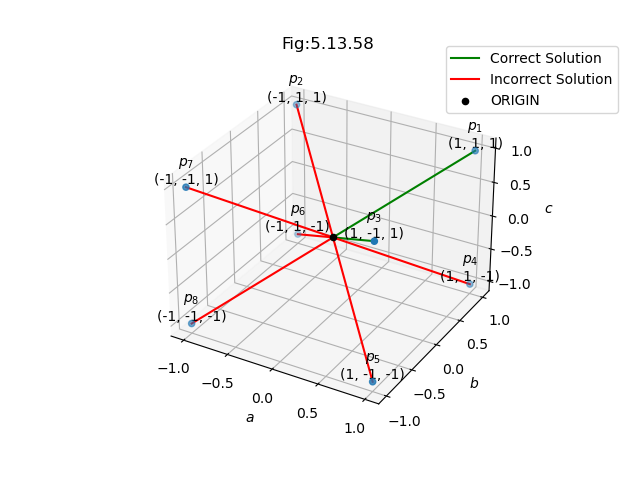
\includegraphics[width=\columnwidth, height=0.8\textheight, keepaspectratio]{../figs/vector1.png}   
\end{frame}

\end{document}
